
%(BEGIN_QUESTION)
% Copyright 2015, Tony R. Kuphaldt, released under the Creative Commons Attribution License (v 1.0)
% This means you may do almost anything with this work of mine, so long as you give me proper credit

Sketch wires connecting these multi-ratio CTs to the three ammeters, and also insert screws into the shorting terminal blocks as appropriate, in order to provide a 200:5 CT ratio on each phase:

$$\includegraphics[width=15.5cm]{i01029x01.eps}$$

Assume each of the multi-ratio CTs has the following number of wire turns between terminal pairs:

\begin{itemize}
\item{} 10 turns between X1 and X2
\item{} 5 turns between X2 and X3
\item{} 25 turns between X3 and X4
\item{} 20 turns between X4 and X5
\end{itemize}


\vfil 

\underbar{file i01029}
\eject
%(END_QUESTION)





%(BEGIN_ANSWER)

This is a graded question -- no answers or hints given!
 
%(END_ANSWER)





%(BEGIN_NOTES)

The desired current ratio is 200:5, which is equivalent to 40:1.  Therefore, we need to select a pair of terminals on each CT providing 40 (total) turns.  This can only be X1-X4, with 10+5+25 turns.  Two grounding screws must be inserted into each shorting terminal block: one to bond the shorting bar to ground, and the other to connect one of the CT secondary terminals to ground (typically this is the higher-numbered terminal of the two driving the instrument: in this case, X4).

$$\includegraphics[width=15.5cm]{i01029x02.eps}$$

%INDEX% Protective relay: shorting terminal block

%(END_NOTES)


